\documentclass[tikz,border=2pt]{standalone}
\usetikzlibrary{calc}
\usetikzlibrary{intersections}
\usetikzlibrary{patterns}
\usepackage{bm}
\usetikzlibrary{positioning}
\usetikzlibrary{shapes}
\usepackage{pgfplots}
\pgfplotsset{compat=1.18}

\begin{document}

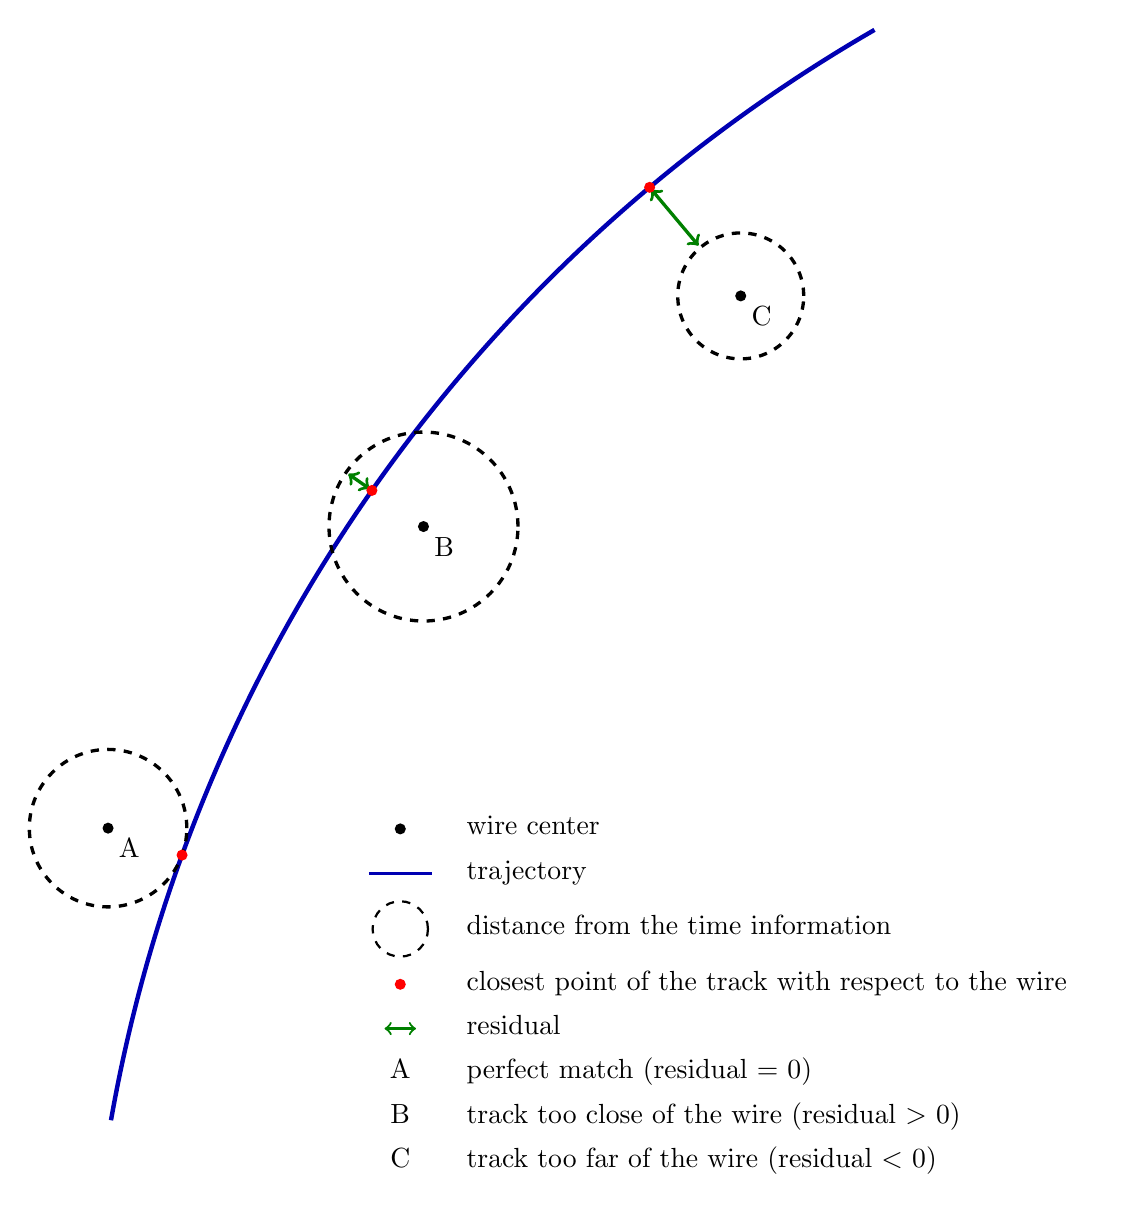
\begin{tikzpicture}[very thick]
    % \tikzset{
    %     every node/.style={font=\scriptsize}
    % }
    
    % ---- Notes ----
    % Track : portion of circle
    % Equation : y = 
    % 

    % Constants
    \pgfmathsetmacro{\xzero}{0}
    \pgfmathsetmacro{\yzero}{0}
    \pgfmathsetmacro{\R}{20}

    % Path
    \draw [ultra thick, blue!70!black] ($(\xzero, \yzero) + (170:\R)$) arc[radius=\R, start angle=170, end angle=120];

    % Control points on the track
    \coordinate (O) at (\xzero, \yzero);
    \coordinate (A) at ($(O) + (160:\R)$);
    \coordinate (B) at ($(O) + (145:\R)$);
    \coordinate (C) at ($(O) + (130:\R)$);


    % \fill (A) circle [radius=2pt];
    % \fill (B) circle [radius=2pt];
    % \fill (C) circle [radius=2pt];
    % \fill (D) circle [radius=2pt];

    % Points on the distance circles
    \coordinate (Ad) at ($(O)!1.05!(A)$);
    \coordinate (Bd) at ($(O)!0.96!(B)$);
    \coordinate (Cd) at ($(O)!0.91!(C)$);


    \draw [dashed] (Ad) circle [radius=0.05*\R];
    \fill (Ad) circle [radius=2pt];

    \draw [dashed] (Bd) circle [radius=0.06*\R];
    \fill (Bd) circle [radius=2pt];

    \draw [dashed] (Cd) circle [radius=0.04*\R];
    \fill (Cd) circle [radius=2pt];



    % correction arrows
    \draw [green!50!black,<->, shorten <=1pt, shorten >=1pt] ($(O)!1.02!(B)$) -- (B);
    \draw [green!50!black,<->, shorten <=1pt, shorten >=1pt] ($(O)!0.95!(C)$) -- (C);

    
    % r > 0 --> rotate to the left
    % r < 0 --> rotate to the right

    % Measurement points
    \fill [red] (A) circle [radius=2pt];
    \fill [red] (B) circle [radius=2pt];
    \fill [red] (C) circle [radius=2pt];


    \node [below right] at (Ad) {A};
    \node [below right] at (Bd) {B};
    \node [below right] at (Cd) {C};

    % \node [draw,align=left, inner sep=8pt, line width=0.5pt] at (-10,5) {
    %     $r > 0$ -- rotate to the right \\
    %     $r < 0$ -- rotate to the left \\
    %     {\color{black} -- } initial layer postion \\
    %     {\color{red} - -} corrected layer position
    %     };

    \newcommand{\distanceline}{\tikz[baseline=-0.5ex] \draw[thick, dashed] (0,0) circle [radius=10pt];}
    \newcommand{\residualline}{\tikz[baseline=-0.5ex] \draw[green!50!black, thick,<->] (0,0) -- (0.4,0);}
    \newcommand{\trackline}{\tikz[baseline=-0.5ex] \draw[very thick,blue!70!black] (0,0) -- (0.8,0);}
    \newcommand{\measurementpoint}{\tikz[baseline=-0.5ex] \fill[red] (0,0) circle [radius=2pt];}
    \newcommand{\wirepoint}{\tikz[baseline=-0.5ex] \fill (0,0) circle [radius=2pt];}

    %\node[draw, rectangle, thin, dashed] at (-12,5) {
    \node at (-12,5) {
        \begin{tabular}{cl}
            \wirepoint  & wire center   \\[4pt]
            \trackline   & trajectory   \\[4pt]
            \distanceline   & distance from the time information  \\[8pt]
            \measurementpoint  & closest point of the track with respect to the wire  \\[4pt]
            \residualline   & residual \\ [4pt]
            A  & perfect match (residual $=$ 0) \\[4pt]
            B  & track too close of the wire (residual $>$ 0)\\[4pt]
            C  & track too far of the wire (residual $<$ 0)\\[4pt]
        \end{tabular}
    };



\end{tikzpicture}


\end{document}